\chapter{KDD Process}

\section{Topic's description}
\subsection{Problem's description}
The objective of a gait pattern recognition system for injury prediction is to accurately identify patterns in an individual's gait (i.e., the way they walk) that may be indicative of an impending injury. This could involve analyzing various aspects of the gait cycle, such as stride length, cadence, and foot placement, and using various algorithm algorithms to identify patterns that are associated with increased risk of injury. The ultimate goal of such a system would be to enable early detection of injuries, potentially reducing the likelihood and severity of injuries for individuals who are at risk.

\bigskip

Inertial measurement units (IMUs) are used to measure motion and orientation. They often have accelerometers, gyroscopes, and magnetometers, but we only need the accelerometer data. In gait pattern recognition, IMUs measure the acceleration and angular velocity of body segments (e.g., lower leg, thigh) as a person walk. This data can extract gait cycle features, such as stride length, cadence, and foot placement, that can indicate an impending injury.

\bigskip

Therefore, using this gait analysis, the following fundamental injuries can be predicted: Balance disorders, Ankle Sprain, and Plantar Fasciitis. And, the target users for this gait pattern analysis are those working in healthcare, such as hospitals, rehabilitation centers, sports teams and athletic trainers, and nursing homes for the elderly. Nonetheless, it is critical to remember that gait pattern analysis is just one tool they can use to predict injuries, and it is not always full proof. In addition, this gait analysis system was designed with all requirements and considerations of RAMI4.0 in mind.


\section{Database}
\subsection{What is the data}
\label{subsection: what is the data}

Acceleration signals along the three axes and timing data are measured in seconds and meters per second, respectively, for each gait phase. Three parameters can be used to evaluate the amount of data for a single research participant: the number of given steps, the number of Gait Phase Data sets, and the number of axes for each gait phase. These three parameters make up the total amount of data \ref{eqn:2.1}

\begin{equation}
\label{eqn:2.1}
    Total\:Data = N_{Step} \times N_{Gait} \times N_{Axis}
\end{equation}
where: 

$N_{Step}$ = Number of given step

$N_{Gait}$ = Number of Gait Phase Data set (HS, TS, HO, TO), represented by 4.

$N_{Axis}$ = Number of axis for each gait phase (X, Y, Z), represented by 6.

\subsubsection{Number of given step}
\label{subsubsection: Number of given step}

In a gait study, data volume and forecast accuracy must be balanced. Collect more data to learn stable, transferrable patterns for machine learning. Collecting enough data to make accurate projections is expensive and risky. Finding the optimal data volume-prediction accuracy balance may require experimentation.

\bigskip

Unfortunately, we're only starting analysis, not execution. An average-sized person will need 1,408 steps to walk one kilometer at a normal pace, according to a study in the Health \& Fitness Journal of the \ac{acsm}. Therefore, we decide to apply 1408 total steps to pur analysis. \cite{Hoeger2008}

\subsubsection{Number of Gait Phase Data sets}

Gait phases will be analyzed as heel strike (HS), toe strike (TS), heel-off (HO), and toe-off (TO). By declaring 4 gait phase data sets, it is clear that data will be collected for each phase. This approach allows for a more detailed and comprehensive gait pattern analysis, which can help predict balance disorders or injuries like ankle sprains or plantar fasciitis.

\subsubsection{Number of axes for each gait phase}
By evaluating the x-axis acceleration data, the forward or backward body movement during gait can be determined. By evaluating acceleration data along the y-axis, one may identify body movement during walking. By evaluating z-axis acceleration data, one can tell whether the body moves uphill or downward during gait. Thus providing a more complete picture of the gait pattern that can be used to predict balance problems or injuries like ankle sprains or plantar fasciitis.

\subsection{How to reach the data}
The data is collected from the sensor using Bluetooth. Then in a Python environment we set the rate that the information will be taken out of the sensor, in our case 200Hz from the accelerometer and next we open a serial connection to the Portenta H7's serial port. Once this is done we gather the sensor data in an array in python with a time stamp so is possible to operate with the information as a function of the acceleration on each axis through time.

\section{Data Selection}

\bigskip

Data selection in the KDD process refers to the process of identifying and selecting the specific data that will be used in the analysis. This could include selecting specific records or subsets of the data based on certain criteria, such as the type of injury or the specific gait patterns being analyzed, Therefore in this section, we are describing the information regard two topic

\subsection{Selection of injury's type}
%%we are going to describe what is it the of injury we are going to predict here

A person's walking pattern, or gait analysis, can be used to spot and treat a number of ailments and injuries. Three of the several instances include Balance disorders, Ankle Sprain, and Plantar Fasciitis
\begin{itemize}
 
\item \textbf{Balance disorders}: \\
Several variations in walking style may result from a balance disorder. If a person has trouble keeping their balance while standing or walking, they may try to adjust their gait to feel more stable.

\item \textbf{Ankle Sprain}: \\
An ankle sprain is an injury that happens when the ligaments in the ankle are stretched or torn. This injury can occur when the ankle is suddenly turned or twisted or when the person lands awkwardly on the ankle. Sprained ankles can hurt, swell, and make it hard to walk or stand on the affected foot.

\item \textbf{Plantar Fasciitis} \\
Plantar fasciitis is a common cause of heel pain that is characterized by inflammation of the plantar fascia, a thick band of tissue that runs along the bottom of the foot from the heel to the toes. Plantar fasciitis can cause pain and difficulty walking, particularly first thing in the morning or after prolonged standing or walking periods.


\end{itemize}

\subsection{Selection of Specific gait pattern}
\label{subsection:Selection of Specific gait pattern}

First of all, once we have the raw data, an analysis of it is not needed to be done directly on the first place, as it is possible to do a division between the steps that are being done by the same foot (as we are talking about the analysis of the signals made by the sensors of one foot only) by looking at the flat phases of the representation of $\ddot{z}_h$ or $\ddot{z}_t$, or by checking the periods where the value of one of them is 0, meaning that the heel or the toe in that moment it is touching the ground, this defining a "heel flat phase" or "toe flat phase" \cite{Mohamed2015}.

\begin{figure}[h]
    \centering
    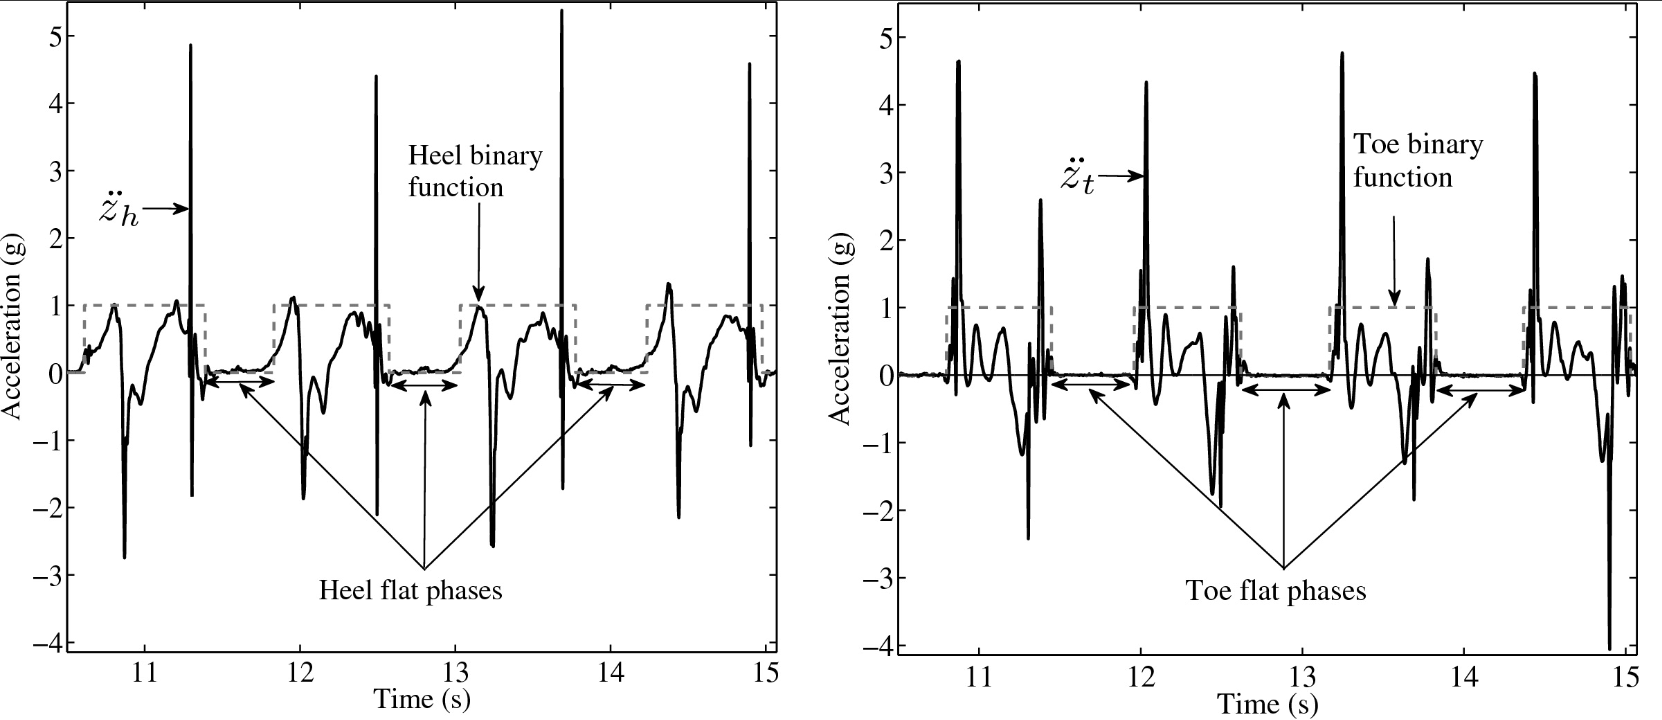
\includegraphics[scale=0.2]{Images/flat-phases.png}
    \captionsetup{justification=centering}
    \caption{Flat phases represented by $\ddot{z}_h$ and $\ddot{z}_t$ respectively \\ source: \cite{Mohamed2015}}
    \label{fig:flat-phases}
\end{figure}

\bigskip

Secondly, in order to do a more extensive analysis we separate each step in 4 phases, HS, TS, HO and TO. This separation can help differentiate gait patterns between people, but not enough to discriminate all the features that describe different type of injures or diseases, then we also add valuable data that can help distinguish them: The data measured by the accelerometer in all axis at the moment of each phase, thus helping to know the conditions of the foot at that specific instant, i.E: the straightness of the Heel Strike (HS). 




\section{Data Preparation / Outliers}

\bigskip
\subsection{Data Preparation}
\label{subsection:Data Preparation}
In the Knowledge Discovery in Databases (KDD) process, "data preparation" refers to the steps of cleaning, formatting, and organizing the data that will be used in the analysis. A few examples are eliminating duplicates, dealing with missing values, and normalizing the data range. In contrast, data preparation in the gait injury prediction system is the process that follows the collection of time-recorded data from research participants, which can be broken down into a "heel flat phase" and a "toe flat phase".

\bigskip

Consequently, gait cycle extraction will be performed to get the data ready for the Recurrent Neural Network (RNN). To do so, we must understand that the binary functions representing the heel and toe are produced at this time scale. Therefore, our proposed method employs the Butterworth filter to extract the four gait events of interest from the time intervals during which the accelerometer is in motion by making use of the local information associated with the flat phase boundaries. Each of the four gait events—heel strike (HS), toe strike (TS), heel-off (HO), and toe-off (TO)—can be defined in terms of their corresponding timing in the following way.

\begin{itemize}

  \item \textbf{Heel Strike (HS)}\\
  HS is determined by filtering $\ddot{z}_h$\footnote{The acceleration data in axis Z captured by the IMU sensor on the heel} with a fourth-order zero-lag Butterworth high-pass filter (10 Hz cutoff). HS is the time of the maximum magnitude of the filtered $\ddot{z}_h$\footnotemark[\value{footnote}] in the heel non-flat phase. HS occurs quickly with a frequency greater than 10 Hz, so this filtering step was unnecessary.
  \\
  \item \textbf{Toe Strike (TS)}\\
  TS is found by observing the time at which the raw $\ddot{z}_t$\footnote{The acceleration data in axis Z captured by the IMU sensor on the toe} peaks at its highest and lowest points within the interval bounded by the HS and the lower boundary of the toe flat phase.
  \\
  \item \textbf{Heel-Off (HO)}\\
  Before defining the signal in a sub-interval, the vertical heel acceleration is divided using the toe binary function. The segmented heel signal is filtered using a fourth-order zero-lag Butterworth low-pass filter (20 Hz). The segmented acceleration signal is added twice to get its position signal in the sub-interval. This double integration's drift is limited by its short duration. To estimate the convex curvature in the position signal (the transition regions), we use a piecewise linear fitting method with two linear segments that best fit the signal in the least-squares sense. This procedure is done twice to improve the accuracy of this sub-interval. Lastly, it is assumed that the estimated HO will be at the time location of the convex curvature.
  \\
  \item \textbf{Toe-Off (TO)}\\
  When calculating TO, we take the midpoint between the upper boundary of the toe flat phase and the highest peak of the raw $\ddot{z}_t$\footnotemark[\value{footnote}] during the first half of the toe non-flat phase.
  \\  
\end{itemize}
\subsection{Outliers}
When analyzing gait patterns using an accelerometer, outliers can happen for several reasons. Outliers may have a variety of causes, such as abrupt movements, improper accelerometer placement, and data processing errors.

\bigskip

A \ac{lstm} algorithm is one option for dealing with outliers in the data collected by the accelerometer in the Arduino Portenta H7 IMU for gait pattern analysis (Long Short-Term Memory). LSTM is a type of recurrent neural network that works well with time series data, such as the accelerometer's collected acceleration data.

\bigskip

In order to use LSTM to deal with outliers in acceleration data, one must first pre-process the data to eliminate any extreme values that could be considered outliers. This can be accomplished through the moving median technique.

\bigskip

After pre-processing data, it can be fed into the LSTM model. The LSTM model will analyze the data and identify patterns or trends, which can then be used to identify and filter out remaining outliers. Hence, Using LSTM in conjunction with the moving median technique can efficiently handle outliers in the acceleration data collected by the Arduino Portenta H7 IMU for gait pattern analysis.

\section{Data Transformation}
\label{section:Data Transformation}

In the KDD process, data transformation is the process of transforming the data into a format that is more suitable for further analysis, which in our case is a Recurrent neural network. Therefore, the gait injury prediction system's data transformation will include aggregation and feature extraction, which can help extract more meaningful patterns and trends from the data.

\bigskip

Regarding subsection: \ref{subsection: what is the data}, we mentioned that the amount of data we are evaluating for a single research participant should be evaluated based on three parameters. Nonetheless, there are a total of 33,738 data items that must be reduced at some point. Consequently, we will use feature extraction to convert unprocessed data into numerical features that can be fed into a Recurrent Neural Network (RNN) while preserving the information in the original data set. In order to accomplish this, we suggest performing two calculations on the data before providing the data mapping. After performing two mentioned calculations, we therefore able to form the data set for individual research participant as follow table \ref{table:Format of dataset for one research participant}


\begin{itemize}
    \item Average time between phases of the same gait phase: For calculate this, we take the information for the gait phases of one of the foot for then calculate the time that has passed between that phase and the next time the same phase take place in a iterative way till we have the sum of all of them, after this we need to divide into the total amount of steps (1408) to get the mean time. We repeat these process with both foot and all gait phases.
    \item Mean of the accelerometer info recorded when each stage of the same gait phase took place: Once again we take the information of the timings where one of the gait phases took place on one foot to then see the value of one axis in all of them and calculate the mean by dividing the sum into the number of recorder steps. We repeat these process with both foot calculating the mean velocity of the 4 phases for each axis.
\end{itemize}

\begin{table}[h!]
\centering
\resizebox{3.5cm}{!}{
\begin{tabular}{ | m{6em} | m{2.1cm}|} 

  \hline
  \multicolumn{2}{|c|}{$Data$}\\
  \hline
  $Parameter$ & $Unit$ \\ 
  \hline
  \hline
  \multicolumn{2}{|c|}{$Person ID$}\\
  \hline
  Weight Height \newline Age & kg \newline m \newline years \\ 
  \hline
  \multicolumn{2}{|c|}{$Gait\:Phase\:Mean$}\\
  \hline
  $HS_{mean}$ $TS_{mean}$ $HO_{mean}$  $TO_{mean}$  & \{s, s\} \\ 
  \hline
  \multicolumn{2}{|c|}{$Velocity\:Xaxis\:Mean$}\\
  \hline
  $V_{HS_{Xmean}}$ $V_{TS_{Xmean}}$ $V_{HO_{Xmean}}$  $V_{TO_{Xmean}}$ & \{m/s, m/s\} \\ 
  \hline
  \multicolumn{2}{|c|}{$Velocity\:Yaxis\:Mean$}\\
  \hline
  $V_{HS_{Ymean}}$ $V_{TS_{Ymean}}$ $V_{HO_{Ymean}}$  $V_{TO_{Ymean}}$ & \{m/s, m/s\} \\ 
  \hline
  \multicolumn{2}{|c|}{$Velocity\:Zaxis\:Mean$}\\
  \hline
  $V_{HS_{Zmean}}$ $V_{TS_{Zmean}}$ $V_{HO_{Zmean}}$  $V_{TO_{Zmean}}$ & \{m/s, m/s\} \\
  \hline

\end{tabular}}
\caption{Format of dataset for one research participant }
\label{table:Format of dataset for one research participant}
\end{table}


\section{Data Mining}

Data mining refers to applying machine learning algorithms and techniques to the data to extract insights and identify patterns and trends. In the context of our injury detection system, we consider a Recurrent Neural Network (RNN) is the most suitable for the acceleration data to diagnose injuries based on gait patterns.

\bigskip
For this task, we are training the Recurrent Neural Network using the TensorFlow library in a Python environment. As input, we will provide the data formatted as shown in Table \ref{table:Format of dataset for one research participant}. About 100 individuals with each of the four output types (balance disorders, ankle sprain, plantar fasciitis, and normal gait) could be sufficient for a reliable prediction. For training the algorithm, we divided the data set into two batches: one containing 80\% of the data and the other containing 20\%. Now, to determine the number of hidden layers in our algorithm, we must consider the size and complexity of the input data, which in our case is extremely large and complex. However, excessive additions can lead to over fitness and slower training. Additionally, we must consider the available size in Portenta H7. Therefore, testing with varying quantities and sizes of layers will be required to determine the optimal combination.

\bigskip

To train the RNN we have to set the neuron data such as the activation function (i.E: for the output, a Sigmoid function activation will be the best for a Multi-class Clasification problem), then for the optimization a good optimizer for multi-class classification problems could be the \ac{sgd} together with a Categorical cross-entropy loss function. We will require some experimentation to find the best configuration for the batch size and the number of epochs. Once the RNN is trained we test it using the test data set for then calculate the accuracy of the algorithm.
\section{Model}
The model in the KDD process refers to the machine learning model that has been trained on the data and is used to make predictions or identify patterns.

\begin{figure}[h]
    \centering
    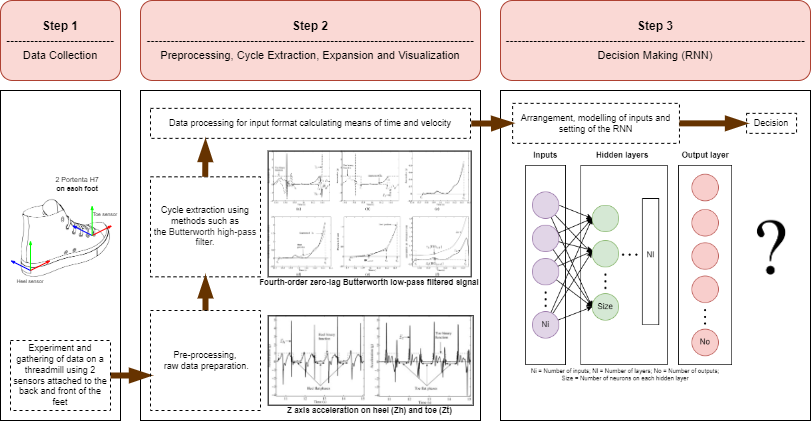
\includegraphics[scale=0.45]{Images/Summary-diagram.png}
    \caption{Summary Diagram}
    \label{fig:Model}
\end{figure}

\section{Validation/Verification}
This would involve evaluating the performance of RNN with the test data, in our case a 20\% of the data set (labeled data), using the sklearn library to show the accuracy of the algorithm predictions. It is also possible to validate it using additional data or methods, such as cross-validation, by splitting the data set into several training and testing sets, so the algorithm's accuracy is not biased by only one training data set, ensuring that it is reliable and accurate. If the accuracy is still low, another kind of readjustment must be done, like normalizing the data.


\section{Model in Production}
Model in production refers to the process of deploying the model in a real-world setting, in our system it involves using the RNN to predict injuries by taking measurements of people walking and then process it to get a diagnosis. For this task it is remarkable the scalability of the method, as we are operating with means it is possible to give more or less steps to get a more reliable output if needed. In terms of security, the information is mostly held in a close environment making it difficult to trespass it to get patient information. Finally, as only 4 sensors are being used, the maintenance part is quite simple, a malfunction of one of them can be easily perceived if too many outliers are being detected coming out of that output on the gait analysis phase. 